\chapter{EXPERIMENTACIÓN COMPUTACIONAL}

Los resultados fueron producidos usando conjuntos de datos sintéticos y reales 
en una máquina
Dell OPTIPLEX 7010 con procesador Intel\textregistered Core\texttrademark  
i7-3770 CPU de 3.40GHz x 8,
16 GB de RAM y 1TB 7200 RPM de Disco Duro, corriendo el Sistema Operativo Debian con linux 3.2. Para 
todos los casos se usaron
los algoritmos implementados en Python, versión 3.

\section{SAN JOAQUIN}

Un grupo de conjuntos de datos sintéticos fueron creados usando un modelo para 
la generación de objetos en movimiento, como se describe en 
\cite{brinkhoff2002framework}.
Dos conjuntos de datos sintéticos fueron creados usando la red de San Joaquín 
proporcionada en el sitio web del generador \cite{Brin:2010:Online}.
El primer conjunto de datos recoge 992140 lugares simulados para 25.000 objetos 
en movimiento durante 60 instantes de tiempo. El segundo recoge 50.000 
trayectorias a partir de 2.014.346 de puntos durante 55 instantes de tiempo. La 
tabla~\ref{tab:datasets}, resume la información principal. Las 
figuras~\ref{fig:SJ25K60} y~\ref{fig:SJ50K55} muestran los tiempos de desempeño 
para estos dos casos de estudio, los parámetros adicionales fueron $\mu$=5, 
$\delta$=3 y  $\mu$=9, $\delta$=3, respectivamente.


\begin{table*}
\caption{Conjunto de datos}
\label{tab:datasets}
\centering
\begin{tabular}{c c r r c}
\toprule
\multirow{2}{*}{Dataset}& \multirow{2}{*}{Red}& \multicolumn{1}{c}{Número de}& 
Número de  & Duración promedio\\
                        &                         & trayectorias & 
\multicolumn{1}{c}{puntos} & de la trayectoria\\
\midrule
SJ25KT60  & San Joaquin & 25000 & 992140  & 40\\
SJ50KT55  & San Joaquin & 50000 & 2014346 & 37\\
TAPAS Cologne  & Cologne, Alemania & 88668 & 3403463 & 38\\
Beijing\_Original   & Beijing, China   & 21573 & 1411846& 65\\
Beijing\_Alternativo   & Beijing, China   & 18700 & 815657 & 43\\
\bottomrule
\end{tabular}\par
\bigskip
\end{table*}

\begin{figure*}
  \centering
  \subfigure[BFE, LCMFlock, FPFlock]{\label{SJ25KT60A} 
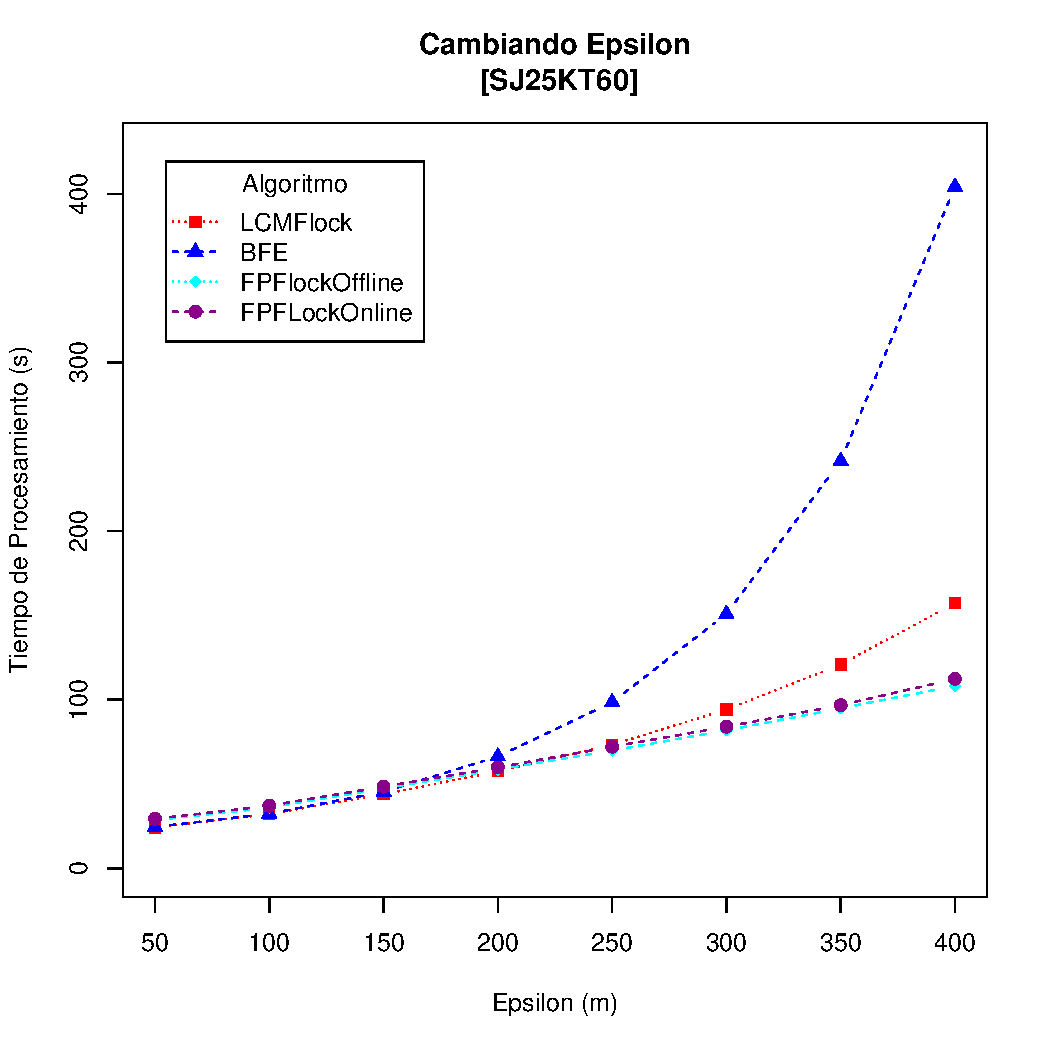
\includegraphics[scale=0.55]{pictures/SJ25KT60.pdf}}
  \subfigure[LCMFlock, 
FPFlock]{\label{SJ25KT60B}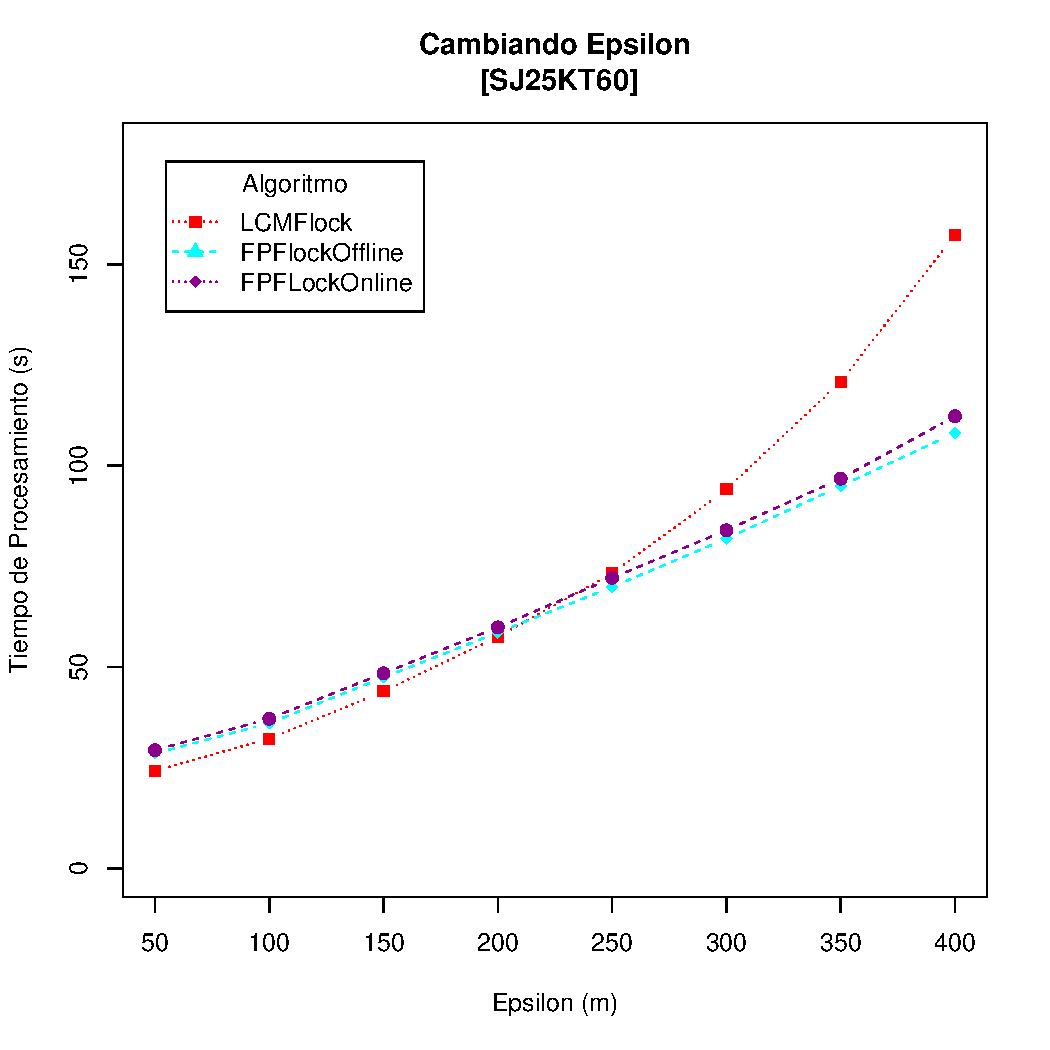
\includegraphics[scale=0.55]{pictures/SJ25KT60_B.pdf}}
  \caption{Caso de Prueba: SJ25KT60. (a) BFE, LCMFlock, FPFlock (b) LCMFlock, FPFlock}
  \label{fig:SJ25K60}
\end{figure*}

\begin{figure*}
  \centering
  \subfigure[BFE, LCMFlock, FP-Flock]{\label{SJ50K55A} 
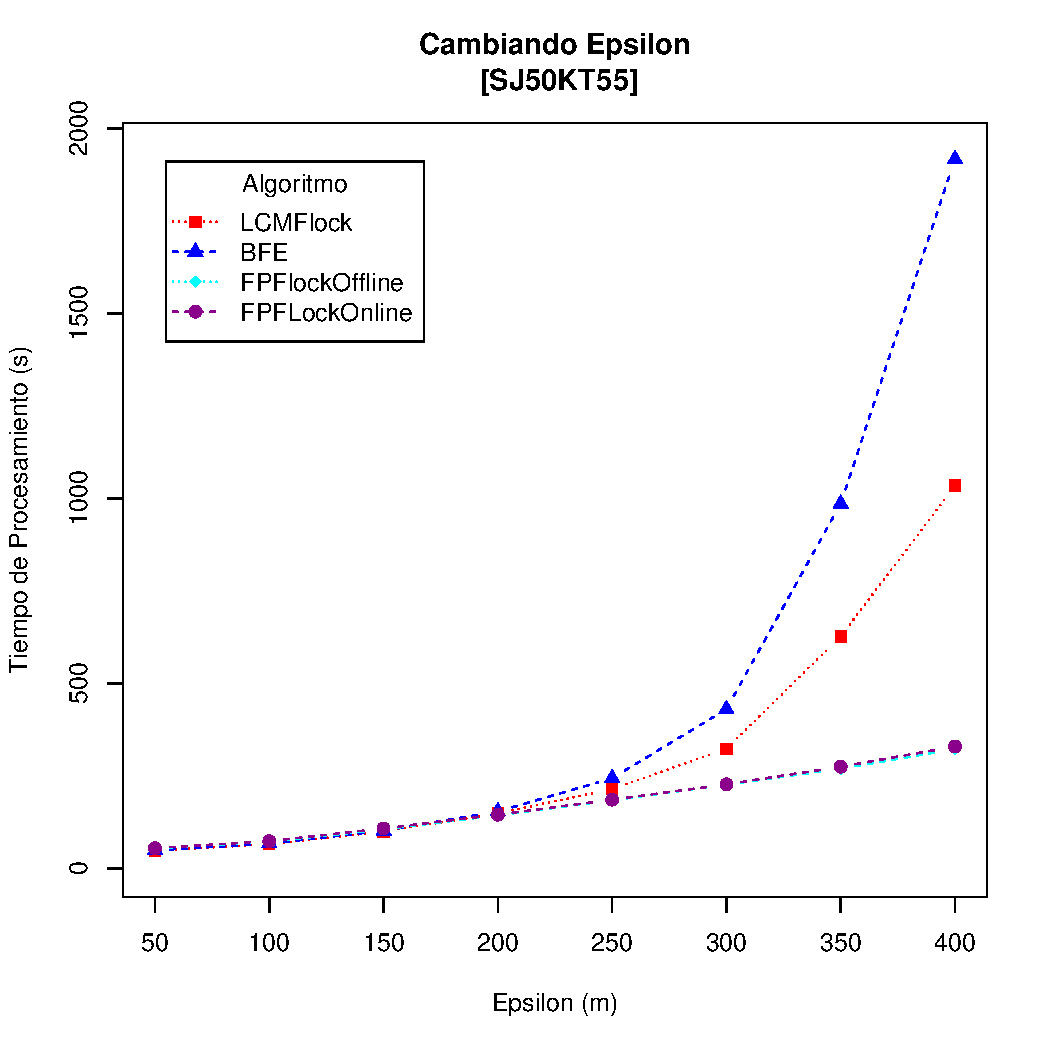
\includegraphics[scale=0.55]{pictures/SJ50KT55.pdf}}
  \subfigure[LCMFlock, FP-Flock]{\label{SJ50K55B} 
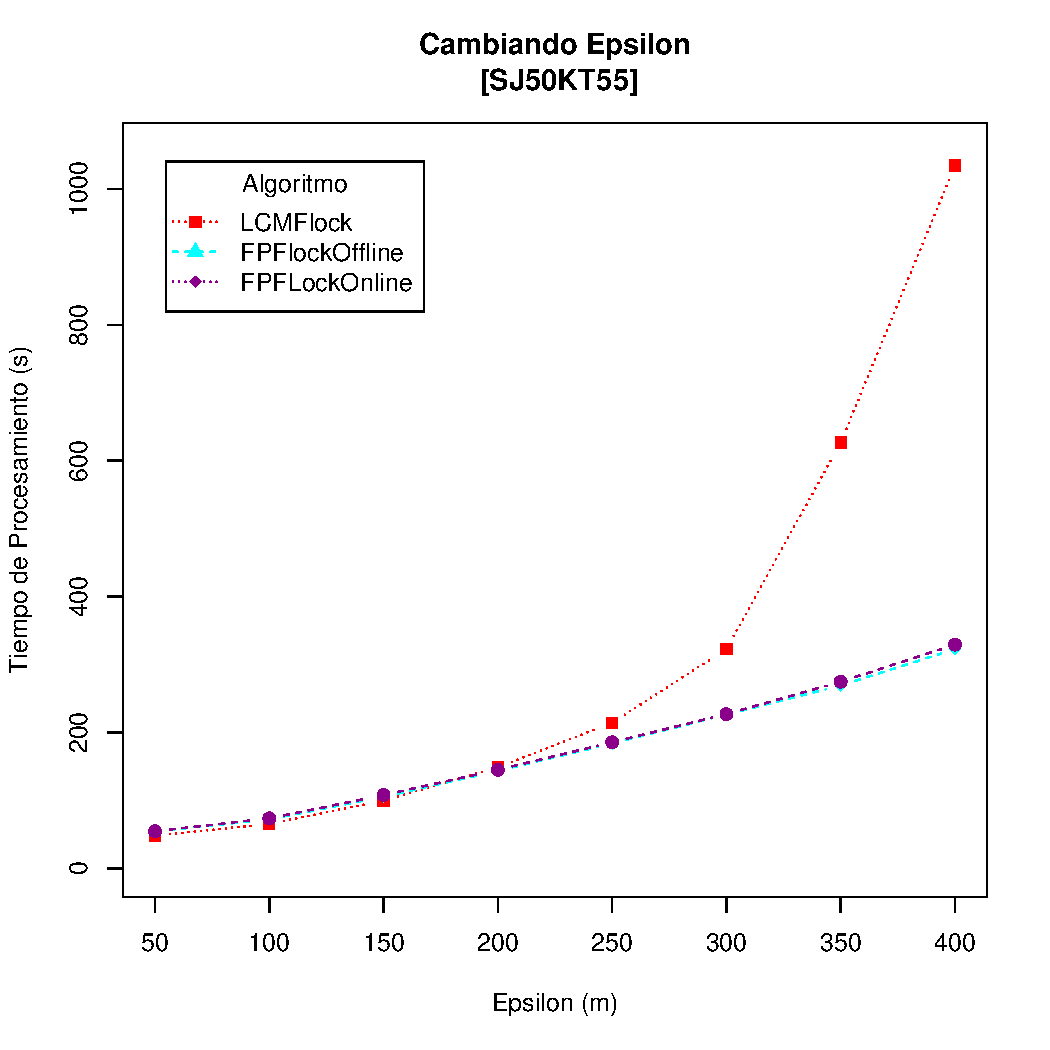
\includegraphics[scale=0.55]{pictures/SJ50KT55_B.pdf}}
  \caption{Caso de Prueba: SJ50KT55. (a) BFE, LCMFlock, FP-Flock (b) LCMFlock, FP-Flock}
  \label{fig:SJ50K55}
\end{figure*}

\section{TAPAS COLOGNE}

Este conjunto de datos sintético se preparó utilizando el escenario TAPAS 
Cologne \cite{varschen2006mikroskopische}
en SUMO \cite{krajzewicz2002sumo}, un reconocido simulador de tráfico para la 
movilidad urbana. El escenario de simulación 
TAPAS Cologne, describe el tráfico dentro de la ciudad de Colonia (Alemania) 
durante un día entero. La principal ventaja de 
este conjunto de datos es que sus trayectorias no se generan aleatoriamente. Los 
datos de la demanda original, se deriva de TAPAS, 
un sistema que calcula la tendencia de movilidad para una población con base en 
la información sobre los hábitos de viaje 
de los alemanes y en la información sobre la infraestructura de la zona en que 
viven \cite{MiD2002}. El conjunto de datos original 
es enorme por lo que sólo está disponible al público la versión de 2 horas 
\cite{TAPASCologne}. Debido a las restricciones de memoria,
se podaron las trayectorias más cortas que 20 minutos. El último conjunto de 
datos recoge 88.668 trayectorias y más 
de 3,4 millones de puntos. La tabla~\ref{tab:datasets}, describe los detalles 
sobre el conjunto de datos. Las figura~\ref{fig:Tapas} muestra los tiempos de 
desempeño para este caso de estudio. Los parámetros adicionales fueron $\mu$=10, 
$\delta$=5.

\begin{figure*}
  \centering
  \subfigure[BFE, LCMFlock, FP-Flock]{\label{tapasA} 
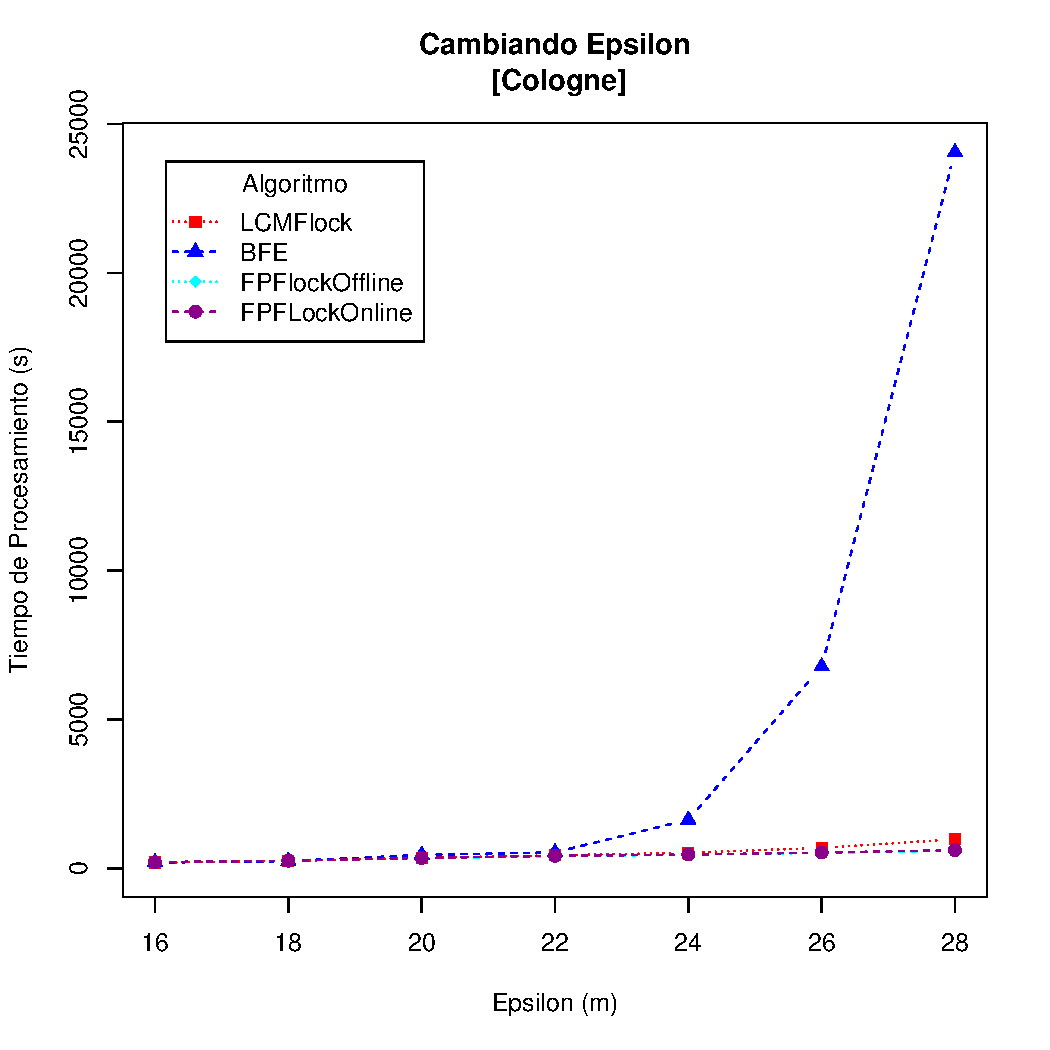
\includegraphics[scale=0.55]{pictures/Cologne.pdf}}
  \subfigure[LCMFlock, FP-Flock]{\label{tapasB} 
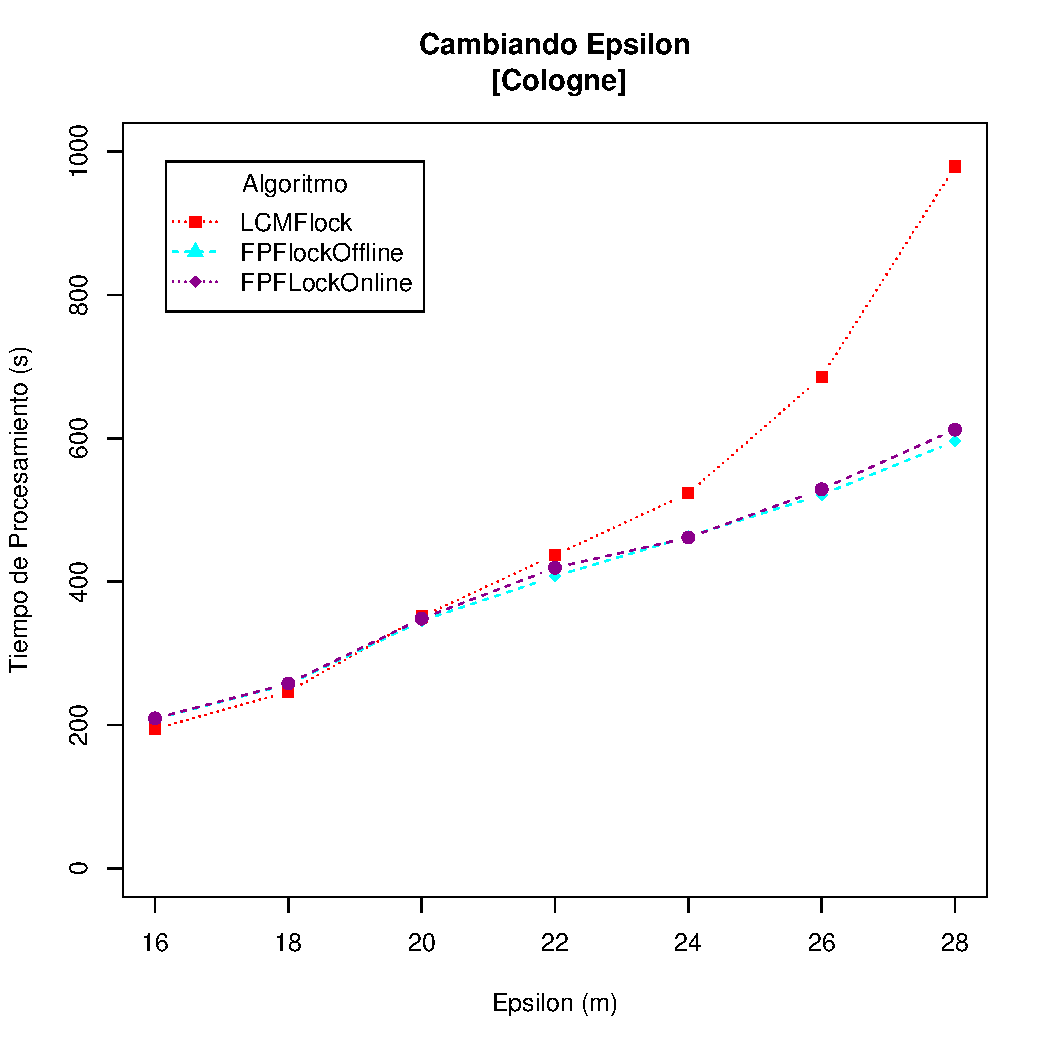
\includegraphics[scale=0.55]{pictures/Cologne_B.pdf}}  
  \caption{Caso de Prueba: Tapas Cologne. (a) BFE, LCMFlock, FP-Flock (b) LCMFlock, FP-Flock}
  \label{fig:Tapas}
\end{figure*}

\section{MOVIMIENTO DE PEATONES EN BEIJING}

Este conjunto de datos reales recopila información de movimiento de un grupo de 
personas en toda
el área metropolitana de Beijing, China\cite{GeoLife}. El conjunto de datos se 
recogió durante el proyecto Geolife por 165 usuarios anónimos en un período de 
dos años entre abril de 2007 y agosto de 2009. Las ubicaciones fueron grabadas 
por diferentes dispositivos GPS o teléfonos inteligentes y la mayoría de ellos 
presentan una frecuencia de muestreo alta. 
La región alrededor del quinto anillo vial en el área metropolitana de Beijing 
mostró la 
mayor concentración de trayectorias. Esto fue usado para generar un conjunto de 
datos de muestra. Cada trayectoria 
fue interpolada por minuto (un punto por minuto) y saltos de 20 minutos o más 
sin señal se utilizaron para marcar una nueva trayectoria. Por último, el 
conjunto de datos recoge más 
de 1,4 millones de puntos y 21.573 trayectorias. Sin embargo, como este conjunto 
de datos tuvo poca cantidad de
entidades en movimiento (165 usuarios) en una ventana de tiempo de más de 2 
años, no existieron muchas trayectorias ocurriendo al mismo tiempo. Para probar
la escalabilidad de los algoritmos, se decidió crear un conjunto de datos alternativo basado en las 
trayectorias reales, pero forzando para que todas ellas comiencen al mismo 
tiempo. Una 
vez más, por las limitaciones de memoria, las trayectorias más cortas que 10 
minutos y más largas que 3 horas se podaron. El conjunto de datos alternativo 
almacenó 815.657 
ubicaciones y 18.700 trayectorias. La tabla~\ref{tab:datasets} resume los 
detalles para ambos conjuntos de datos. Las figuras~\ref{fig:BeijingOr} 
y~\ref{fig:BeijingAl} muestran los tiempos de desempeño para estos dos casos de 
estudio, los parámetros adicionales fueron $\mu$=3, $\delta$=3 y  $\mu$=5, 
$\delta$=5 respectivamente.


\begin{figure}
  \centering
  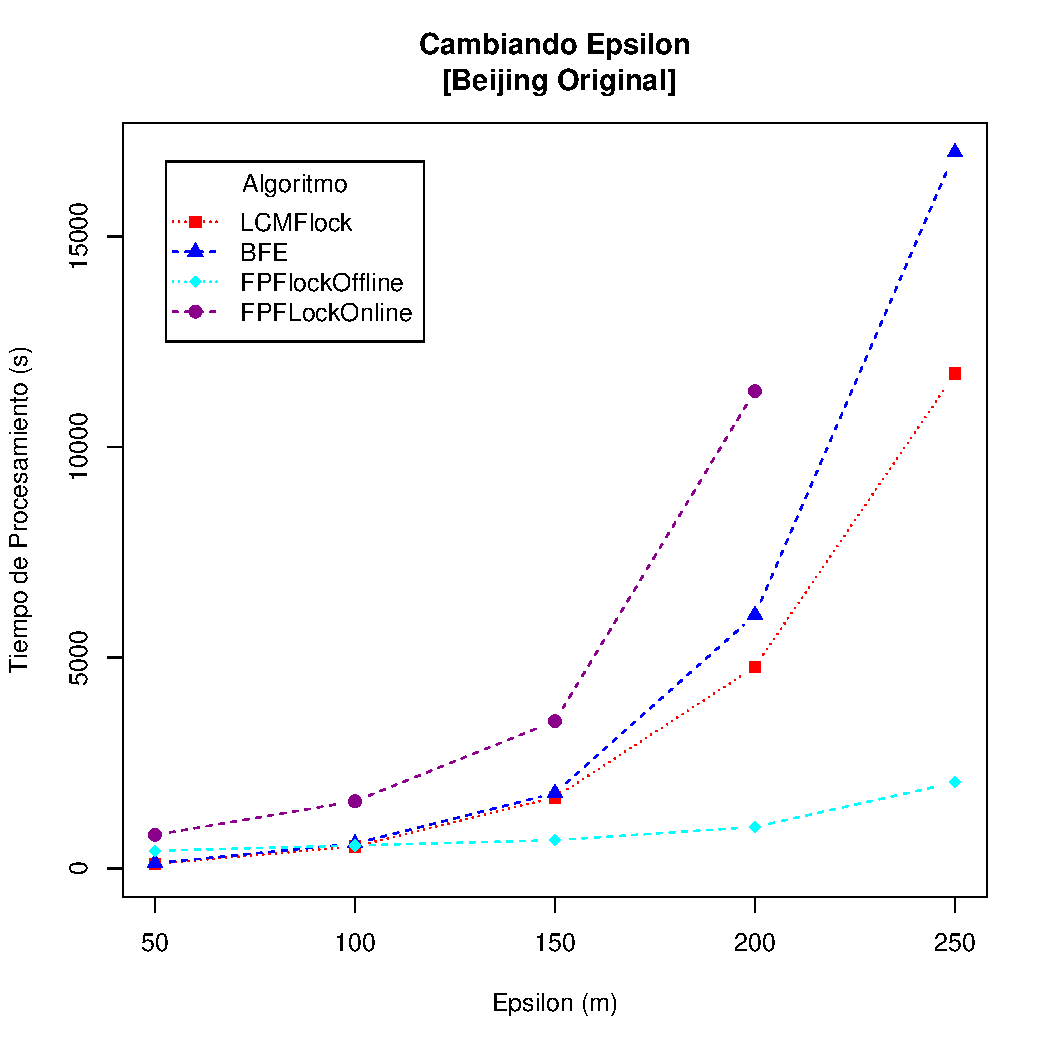
\includegraphics[scale=0.55]{pictures/Beijing_Original.pdf}
  \caption{Caso de Prueba: Beijing Original}
  \label{fig:BeijingOr}
\end{figure}

\begin{figure*}
  \centering
  \subfigure[BFE, LCMFlock, FP-Flock]{\label{b1} 
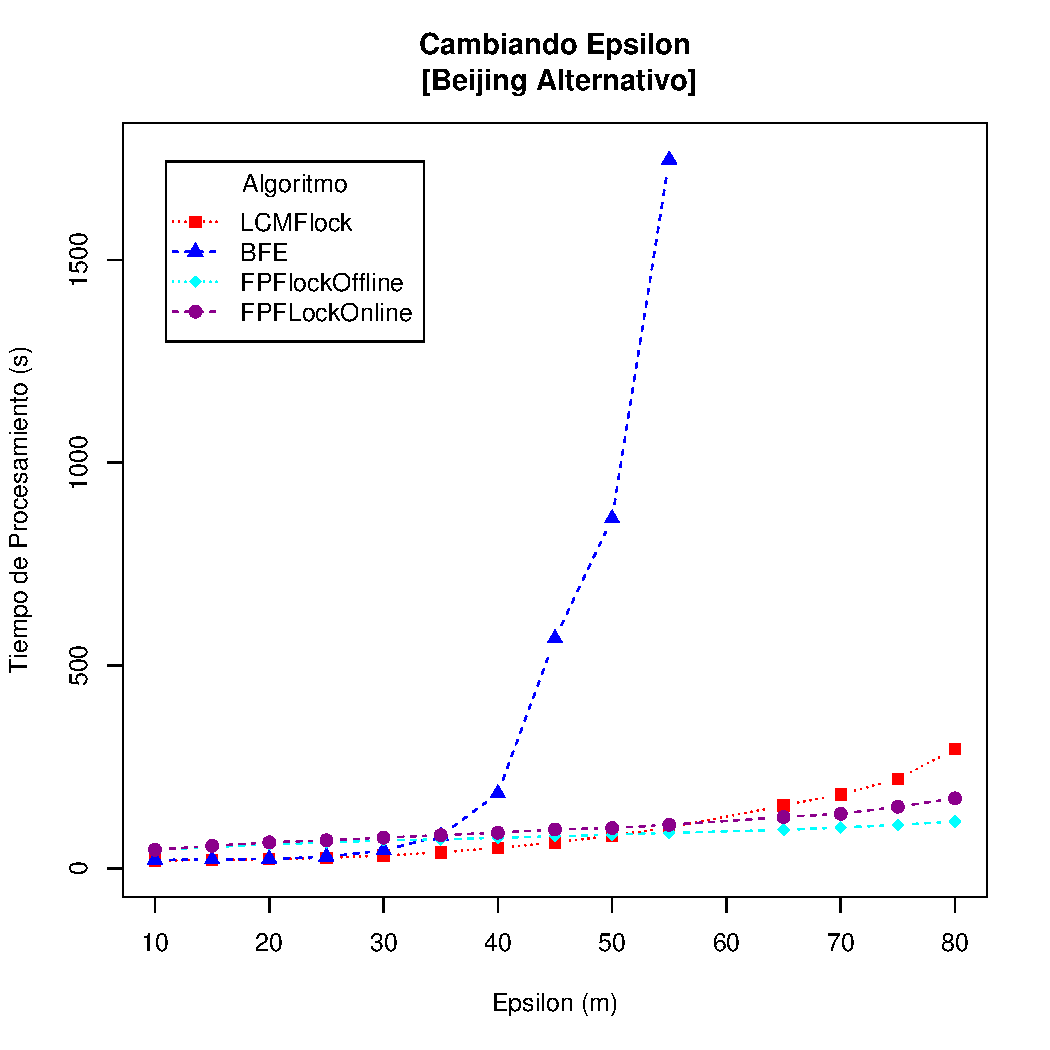
\includegraphics[scale=0.55]{pictures/Beijing_Alternativo.pdf}}
  \subfigure[LCMFlock, FP-Flock]{\label{b2} 
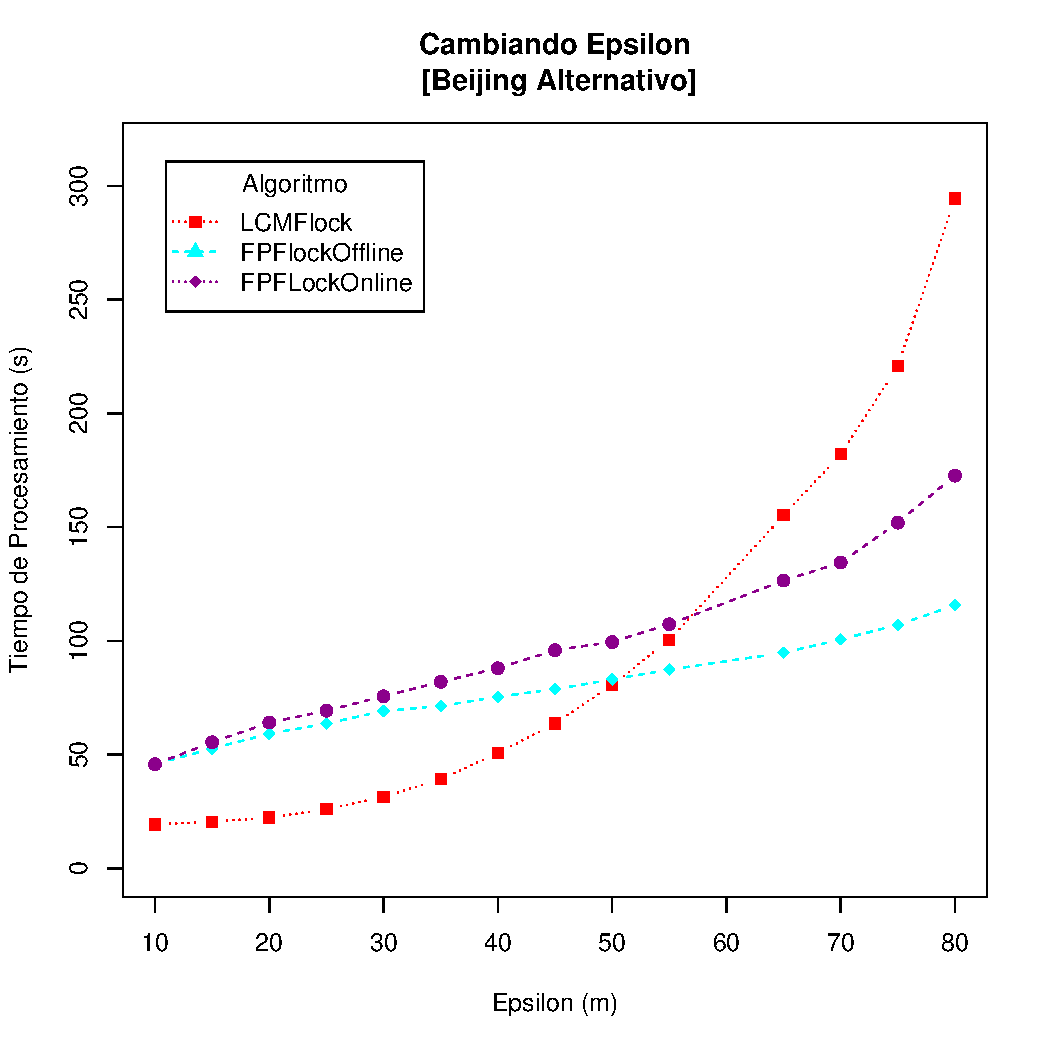
\includegraphics[scale=0.55]{pictures/Beijing_Alternativo_B.pdf}}
  \caption{Caso de Prueba: Beijing Alternativo. (a) BFE, LCMFlock, FP-Flock (b) LCMFlock, FP-Flock}
  \label{fig:BeijingAl}
\end{figure*}


\section{REPORTE DE FLOCKS}

Tanto para BFE, LCMFlock, FP-FlockOnline y FP-FlockOffline el reporte de flocks se hace en una base 
de datos, 
con un identificador, tiempo de inicio, tiempo de fin y todos los puntos 
contenidos en dicho flock. En la tabla~\ref{tab:flocks}, se muestra el número 
total de flocks reportados con un $\varepsilon$ en particular.

\begin{table}
\caption{Número de Flocks}
\label{tab:flocks}
\centering
\scalebox{0.8}{
\begin{tabular}{c c r r r r c}
\toprule
\multirow{2}{*}{Dataset}&  $\varepsilon$ & \multicolumn{1}{c}{Número de Flocks}& Número de Flocks & 
Número de Flocks & Número de Flocks \\
                        &                         &\multicolumn{1}{c}{BFE} & 
\multicolumn{1}{c}{LCMFlock} & \multicolumn{1}{c}{FP-FlockOnline} & 
\multicolumn{1}{c}{FP-FlockOffline}  \\
                        
\midrule
SJ25KT60  & 300 & 35805 & 5466 & 26877 & 5466\\
SJ50KT55  & 300 & 45201 & 6396 & 23638 & 6396\\
TAPAS Cologne  & 28  & 9415451 & 31509 & 145217 & 31509\\
Beijing\_Original   & 250   & 16628029 & 4373139 & - & 4373139\\
Beijing\_Alternativo   & 50   & 6110427 & 19233 & 63566 & 19233\\
\bottomrule
\end{tabular}}\par
\bigskip
\end{table}
